\documentclass[10pt]{article}

\usepackage{times}
\usepackage{graphicx}
\usepackage{url}
\usepackage{color}
\usepackage{multirow}
\usepackage{amsmath}
\usepackage{amssymb}
\usepackage{algorithm}
\usepackage{algorithmicx}
\usepackage{algpseudocode}
\usepackage{cite}
\usepackage{amsthm}
\usepackage{bm}
\usepackage{threeparttable}
\usepackage{geometry}

\geometry{left=2.5cm,right=2.5cm,top=2.5cm,bottom=2.5cm}

\newcommand{\para}[1]{\smallskip\noindent\textbf{#1}}
\newcommand{\etal}{{\em et al.}}

\newtheorem{theorem}{Theorem}
\newtheorem{corollary}{Corollary}
\newtheorem{lemma}{Lemma}
\newtheorem{definition}{Definition}

\begin{document}

%----------------------------------------------------------------------------
\title{\huge Dynamic Channel Deposit and Withdrawl for Lightening Network}
\date{}
\author{LITEX Network}
\maketitle


%----------------------------------------------------------------------------
%\begin{abstract}
\end{abstract}


\section{Introduction}
\label{sec:introduction}


Existing blockchain technology is held back by its serious performance and scalability issues, such as low transaction capacity and prolonged delay. While Bitcoin\cite{nakamoto2008bitcoin} supports less than seven transactions per second, Visa, on the contrary, supports up to 47,000 transactions per second at peak processing power. In Bitcoin, a block is generated every 10 minutes and to ensure the validity of transactions, it requires 6 confirmations, which will take approximately 60 minutes to complete. Bitcoin’s inefficiency and poor scalability inevitably hinder the usability of blockchain in areas such as micropayments.
 
Lightening Network (LN)\cite{poon2015bitcoin} is a practical approach to improve transaction capacity and reduce transaction delay using a network of off-chain micropayment channels\cite{DBLP:journals/corr/LindEPS16}. In LN, any two participants can collectively build a bidirectional off-chain channel by depositing funds into the channel. They can later agree on any new allocation regarding the funds which are already committed to the channel. With a cryptographic technique namely RSMC (Revocable Sequence Maturity Contract), LN guarantees that neither participant has any incentives to deny the latest agreement unless they broadcast their agreement to the main chain. Whomever violates the terms first will lose all of his/her personal funds. In addition to RSMC that ensures unconditional transfer of fundings, LN proposes another mechanism, HTLC (Hashed Timelock Contract), which can be used for conditional transfer. The combination of RSMC and HTLC, together with a large network of micropayment channels on the main blockchain of the Bitcoin network, formed a graph containing all off-chain channels, in which nodes and lines represent participants and off-chain channels respectively. Consequently, participants without mutually shared off-chain channels are still able to make transactions by finding a path connecting different participants between them.

However, several fundamental functionalities and limitations are still left to be developed and improved. One limitation is the malleability of payment channels. In particular, the channel with fixed capacity does not support dynamic deposit and withdrawl, which will result in extra fees for channel management and other possible inconveniences in many scenarios.

Wanting to improve payment channels’ malleability, we address both dynamic channel deposit (a.k.a. splice-in) and withdrawl (a.k.a. splice-out) problems. We have constructed a case to demonstrate that at least one on-chain broadcast is necessary for splice-in and splice-out. We then propose two approaches for splice-in and splice-out that only result in one on-chain broadcast, reducing the number of necessary broadcasts to the minimum.

\section{Background}
\label{sec:problem}

LN allows two counterparties to agree on an off-chain allocation of arbitrary amount of funds. It ensures the off-chain security with the RSMC and HTLC mechanisms.

\begin{figure}[H]
\centering
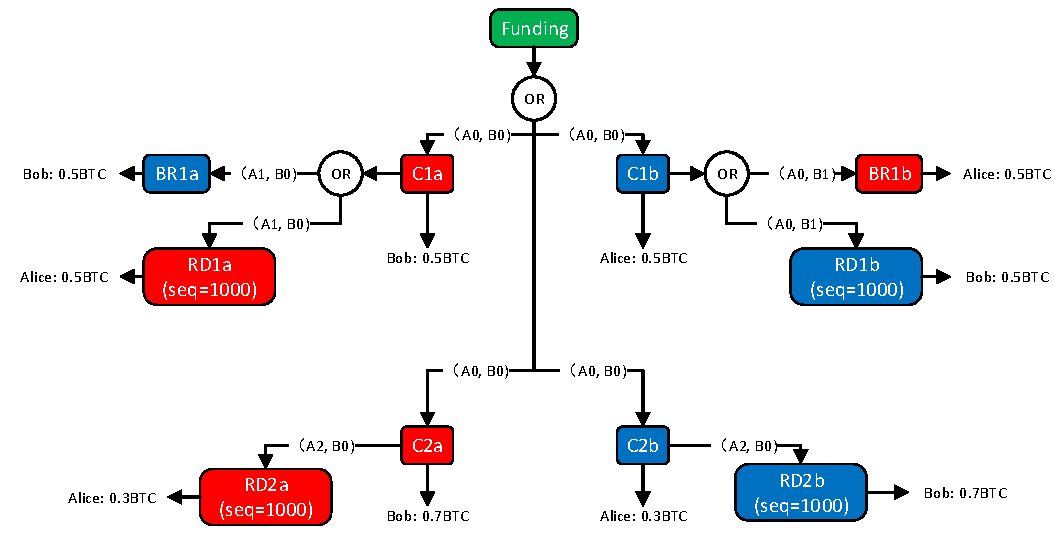
\includegraphics[width=3.5in]{figs/rsmc_old.pdf}
\vspace{-12pt}
\caption{RSMC (Revocable Sequence Maturity Contract)}
\label{fig:RSMC}
\end{figure}


Figure~\ref{fig:RSMC} reviews the RSMC mechanism. RSMC generates a pair of Commitment Transactions, each of which is held by one's counterparty. By broadcasting the Commitment Transaction, a counterparty has the ability to close the channel by spending the Funding Transaction. Accordingly, funds within channel are returned to both counterparties based on their latest agreement. To prevent old Commitment Transaction from being broadcast, RSMC places a LockTime on the funds of the counterparty who broadcasts. At the same time, it also enforces the exchange of private keys between two counterparties for old Commitment Transactions. If either party discovers that an old Commitment Transaction (e.g., C1a in Figure~\ref{fig:RSMC}) is broadcast, he/she can broadcast a penalty transaction (BR1a) with previously exchanged private keys to acquire all funds in the channel. Ensured by this mechanism, no one has the incentive to broadcast old Commitment Transactions.

\begin{figure}[H]
\centering
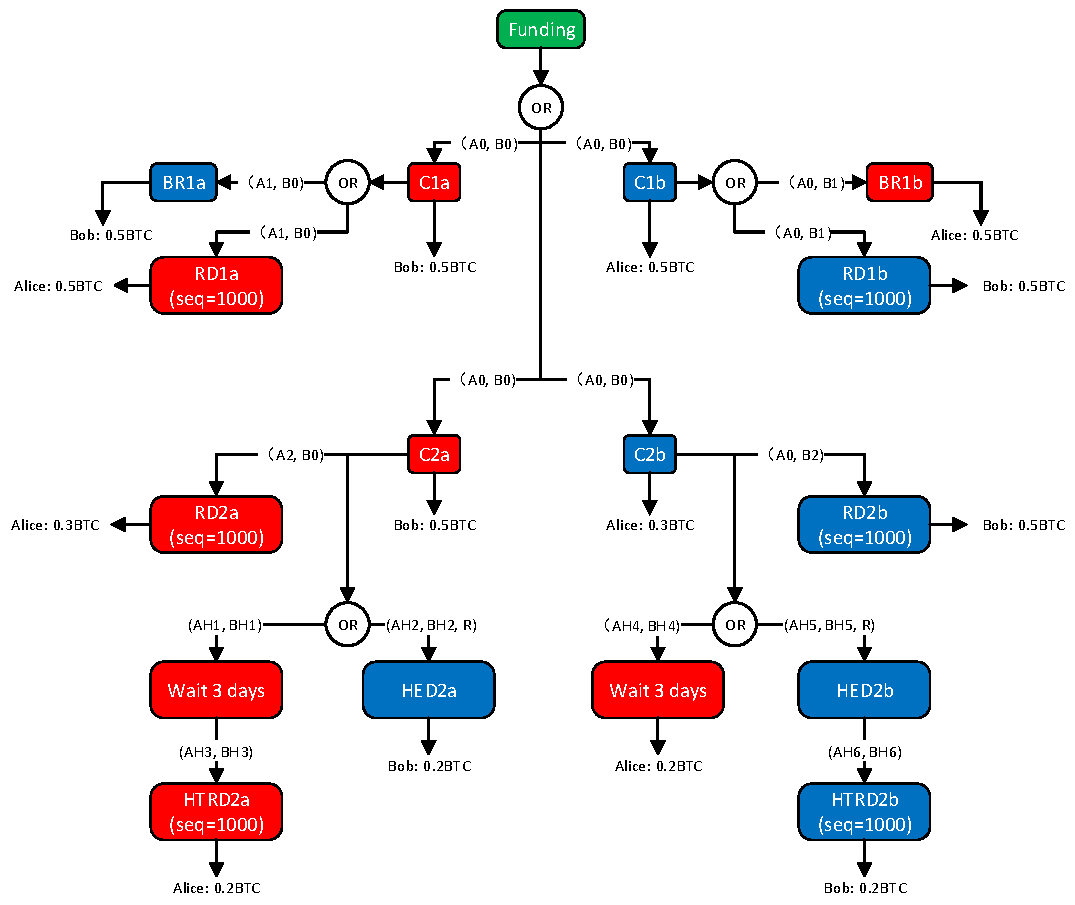
\includegraphics[width=3.5in]{figs/htlc_old.pdf}
\vspace{-12pt}
\caption{HTLC (Hashed Timelock Contract)}
\label{fig:htlc}
\end{figure}


The HTLC mechanism utilizes hash functions, ensured by transactional "locking" between two counterparties, to construct a secure network of channels across multiple destinations between the starting and ending participants\cite{poon2015bitcoin}. Specifically, if the receiver can produce a pre-image $R$ to fulfill a known pre-defined image $H(R)$, the sender pays the receiver. Figure~\ref{fig:htlc} shows the detailed protocol of HTLC, in combination with RSMC to forbid the broadcast of old agreements.


The major limitation of RSMC and HTLC is that funds in the channel cannot be dynamically adjusted unless both participants close and then reopen the channel. Once a channel is built, the total funds in a channel remains fixed. Existing design makes it impossible to deposit new funds into the channel or partially withdraw funds from the channel. Furthermore, the off-chain channel has different capacities in both directions. The capacities continue to change as funds are being transferred between participants, which results in the {\em channel dry-up} problem, meaning funds for that particular direction is exhausted. For instance, assuming one participant is a buyer and the other is a seller, the funds always goes from the buyer to the seller, causing a dry-up in this channel direction. In this case, both participants have to close the channel and recreate a new one. Closing and reopening channels are require to be broadcast, which give rise to extra costs and time delay.


Existing approaches solve the channel dry-up problem by rebalancing funds across multiple channels \cite{Khalil2017}. However, achieving a rebalance requires identification of a loop in the LN graph \cite{Khalil2017}. For example, when the unidirectional channel from A to B dries up, A can find a third-party participant C and transfer some funds to C. Then C transfers the same funds to B (consuming transaction fees). Finally, B transfers the funds back to A, which rebalances the channel between A and B.  This routing-based rebalance requires specific network topology since it is highly probable that no valid loop exists. In a case where a participant is a customer, he/she usually spends his/her channel funds instead of receiving payment from others. Therefore, it is very likely that his/her channels dry up quickly and fails to be rebalanced.


\section{LITEX Solution}
\label{sec:solution}


As we have discussed in \S\ref{sec:problem}, a truly applicable off-chain
architecture needs to support the functionality of dynamical channel deposit and
withdrawl. Original Lightning Network assumes that the total funds in a channel
are throughout the channel's lifetime. Thus, there is no need to broadcast any
in-channel transactions.

\begin{figure}[t]
\centering
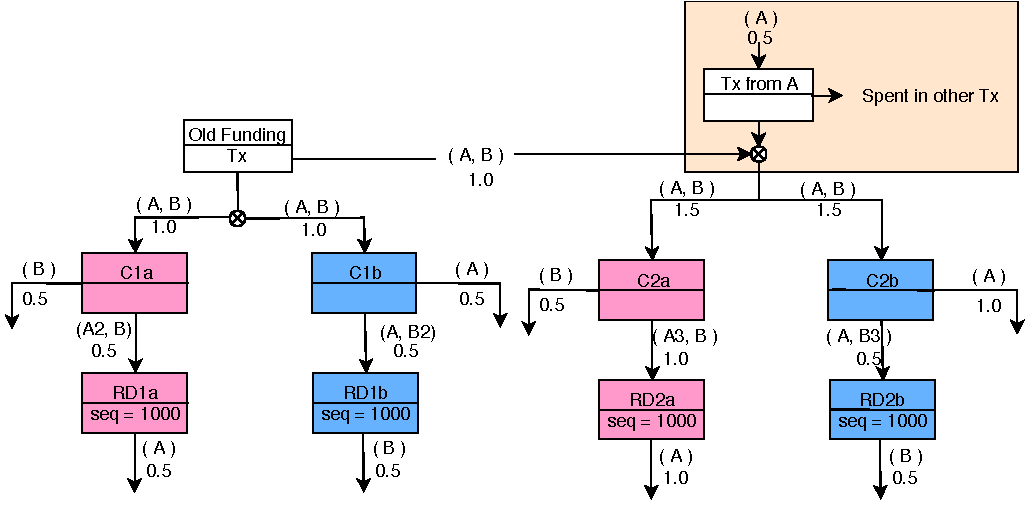
\includegraphics[width=4in]{figs/fake.pdf}
\vspace{-6pt}
\caption{If the deposit from Alice is not broadcasted, she may double spend it after agreement new Committment Transactions with Bob.}
\label{fig:fake}
\end{figure}

\begin{figure}[t]
\centering
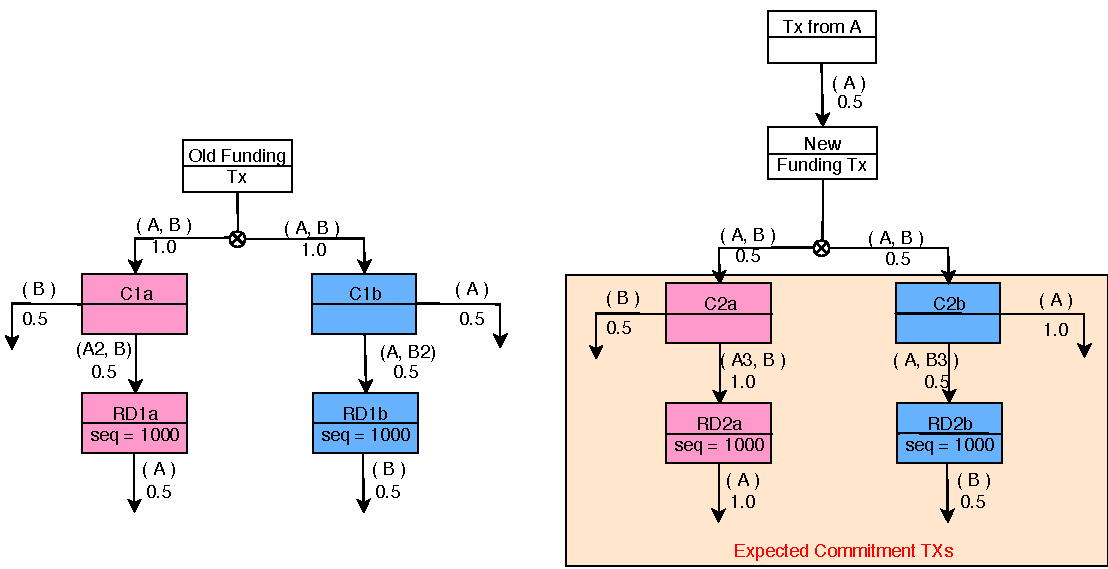
\includegraphics[width=4in]{figs/fund.pdf}
\vspace{-6pt}
\caption{A new Funding Transaction is constructed, the remaining problem is to connect it with old Funding Transaction(s).}
\label{fig:fund}
\end{figure}


When a deposit or a withdrawl occurs, the channel status is modified, which must be verified and recognized by most participants. Otherwise, the counterparty may claim a fake input and double-spend the fund. Figure~\ref{fig:fake} shows an example where Alice deposits 0.5 BTCs into the channel. The deposit results in an agreement on a pair of new Commitment Transactions with her counterparty Bob (1.0 BTC for Alice and 0.5 BTCs for Bob). If the deposit is not broadcast, Alice may spend the fund in other places. Although Bob can detect the double-spend by monitoring all on-chain transactions, he has no method to compensate himself.


Thus, it is necessary to broadcast any channel modification caused by deposit or
withdrawl. To broadcast the channel modification, a new funding transaction has to
be constructed. The channel deposit is shown in Figure~\ref{fig:fund}. In this case, the new Funding Transaction takes an UTXO from an external transaction for deposit. Therefore, broadcasting the funding transaction spends the UTXO so that it cannot be double-spent once the broadcast transaction is verified. The output of the new Funding Transaction is a pair of Commitment Transactions, each of which is held by the respective counterparty in the channel. In Figure~\ref{fig:fund}, the Commitment Transactions also rsult in RD2a and RD2 transactions, which prevent old Commitment Transactions from being broadcast.


The new funding transaction must interact with existing funding transactions to
ensure the validity of new Commitment Transactions. In particular, the total
amount of "vouts" must be equal to that of "vins." We also need to invalidate old Commitment Transactions, i.e., the counterparty who broadcasts any old commitment transaction will lose all his/her funds. Although broadcasting inevitably results in extra costs and delay, it is applicable because channel deposit and withdrawl do not occur frequently.


We now propose two separate approaches to support dynamic channel
deposit (i.e., splice-in) and withdrawl (i.e., splice-out). The two approaches are
differed by the layout of Funding Transactions, and we will elaborate both approaches as follows.

\begin{figure}[t]
\centering
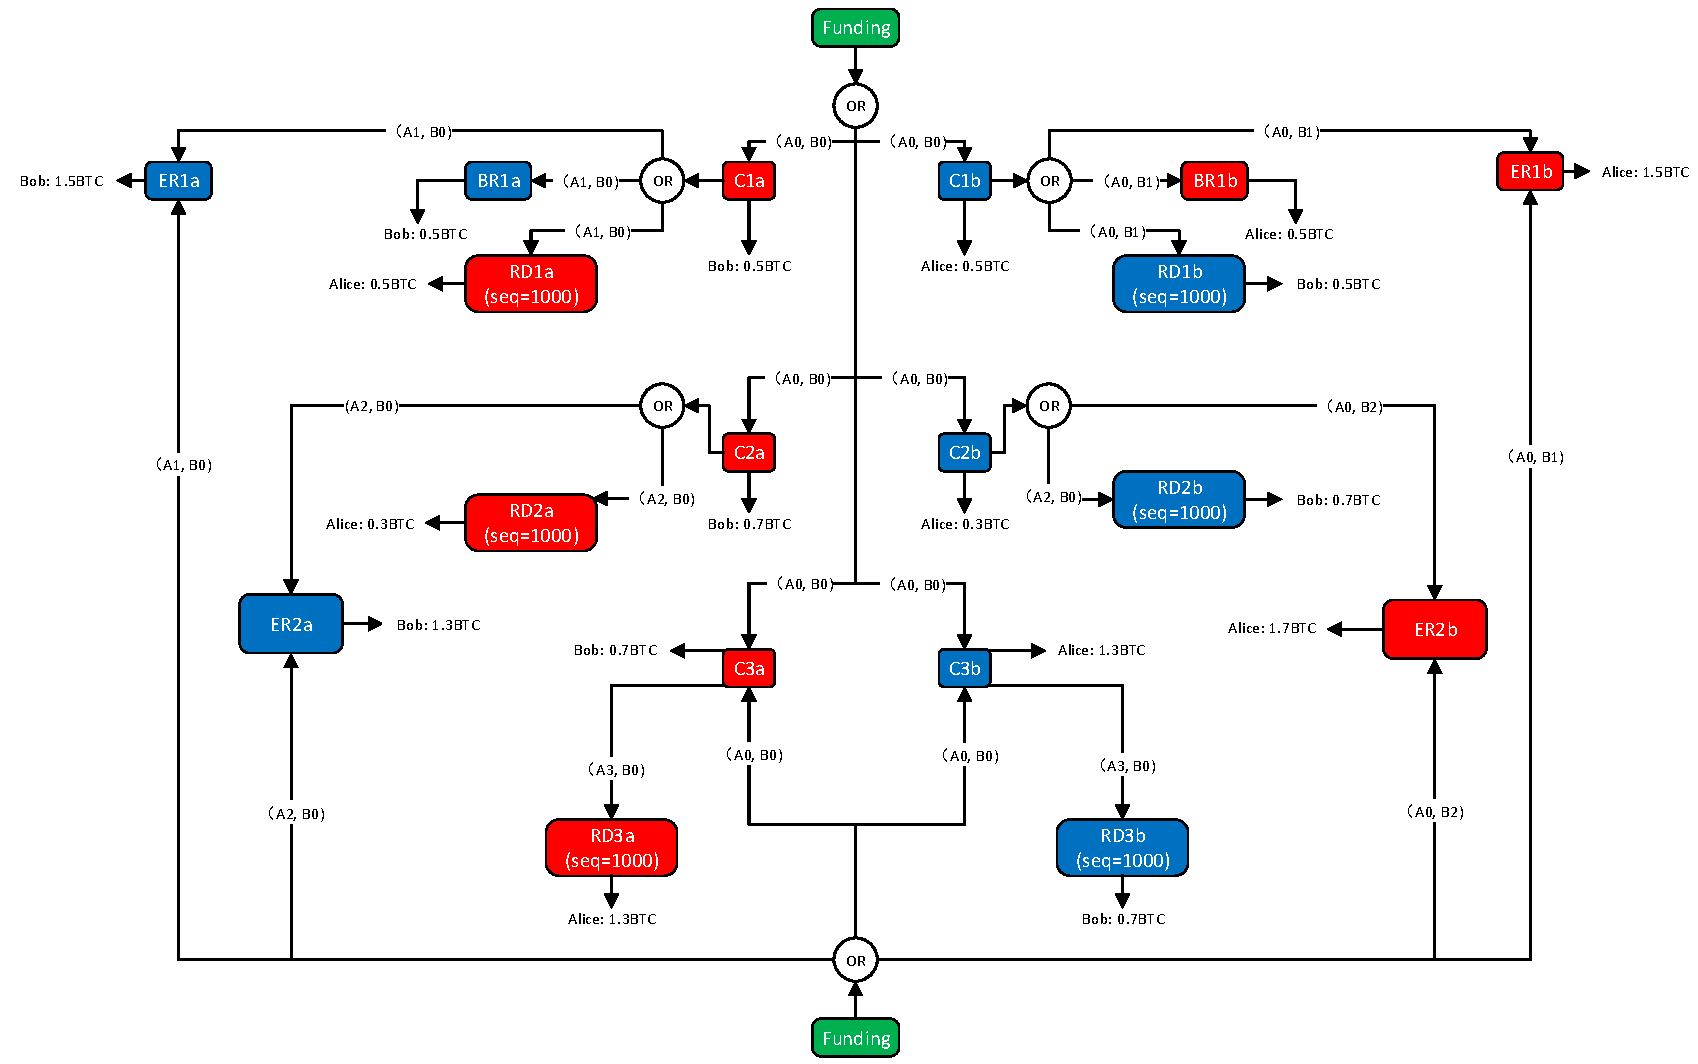
\includegraphics[width=6in]{figs/rsmc_new.pdf}
\vspace{-6pt}
\caption{FundPara RSMC transactions.}
\label{fig:rsmc_new}
\end{figure}

\begin{figure}[t]
\centering
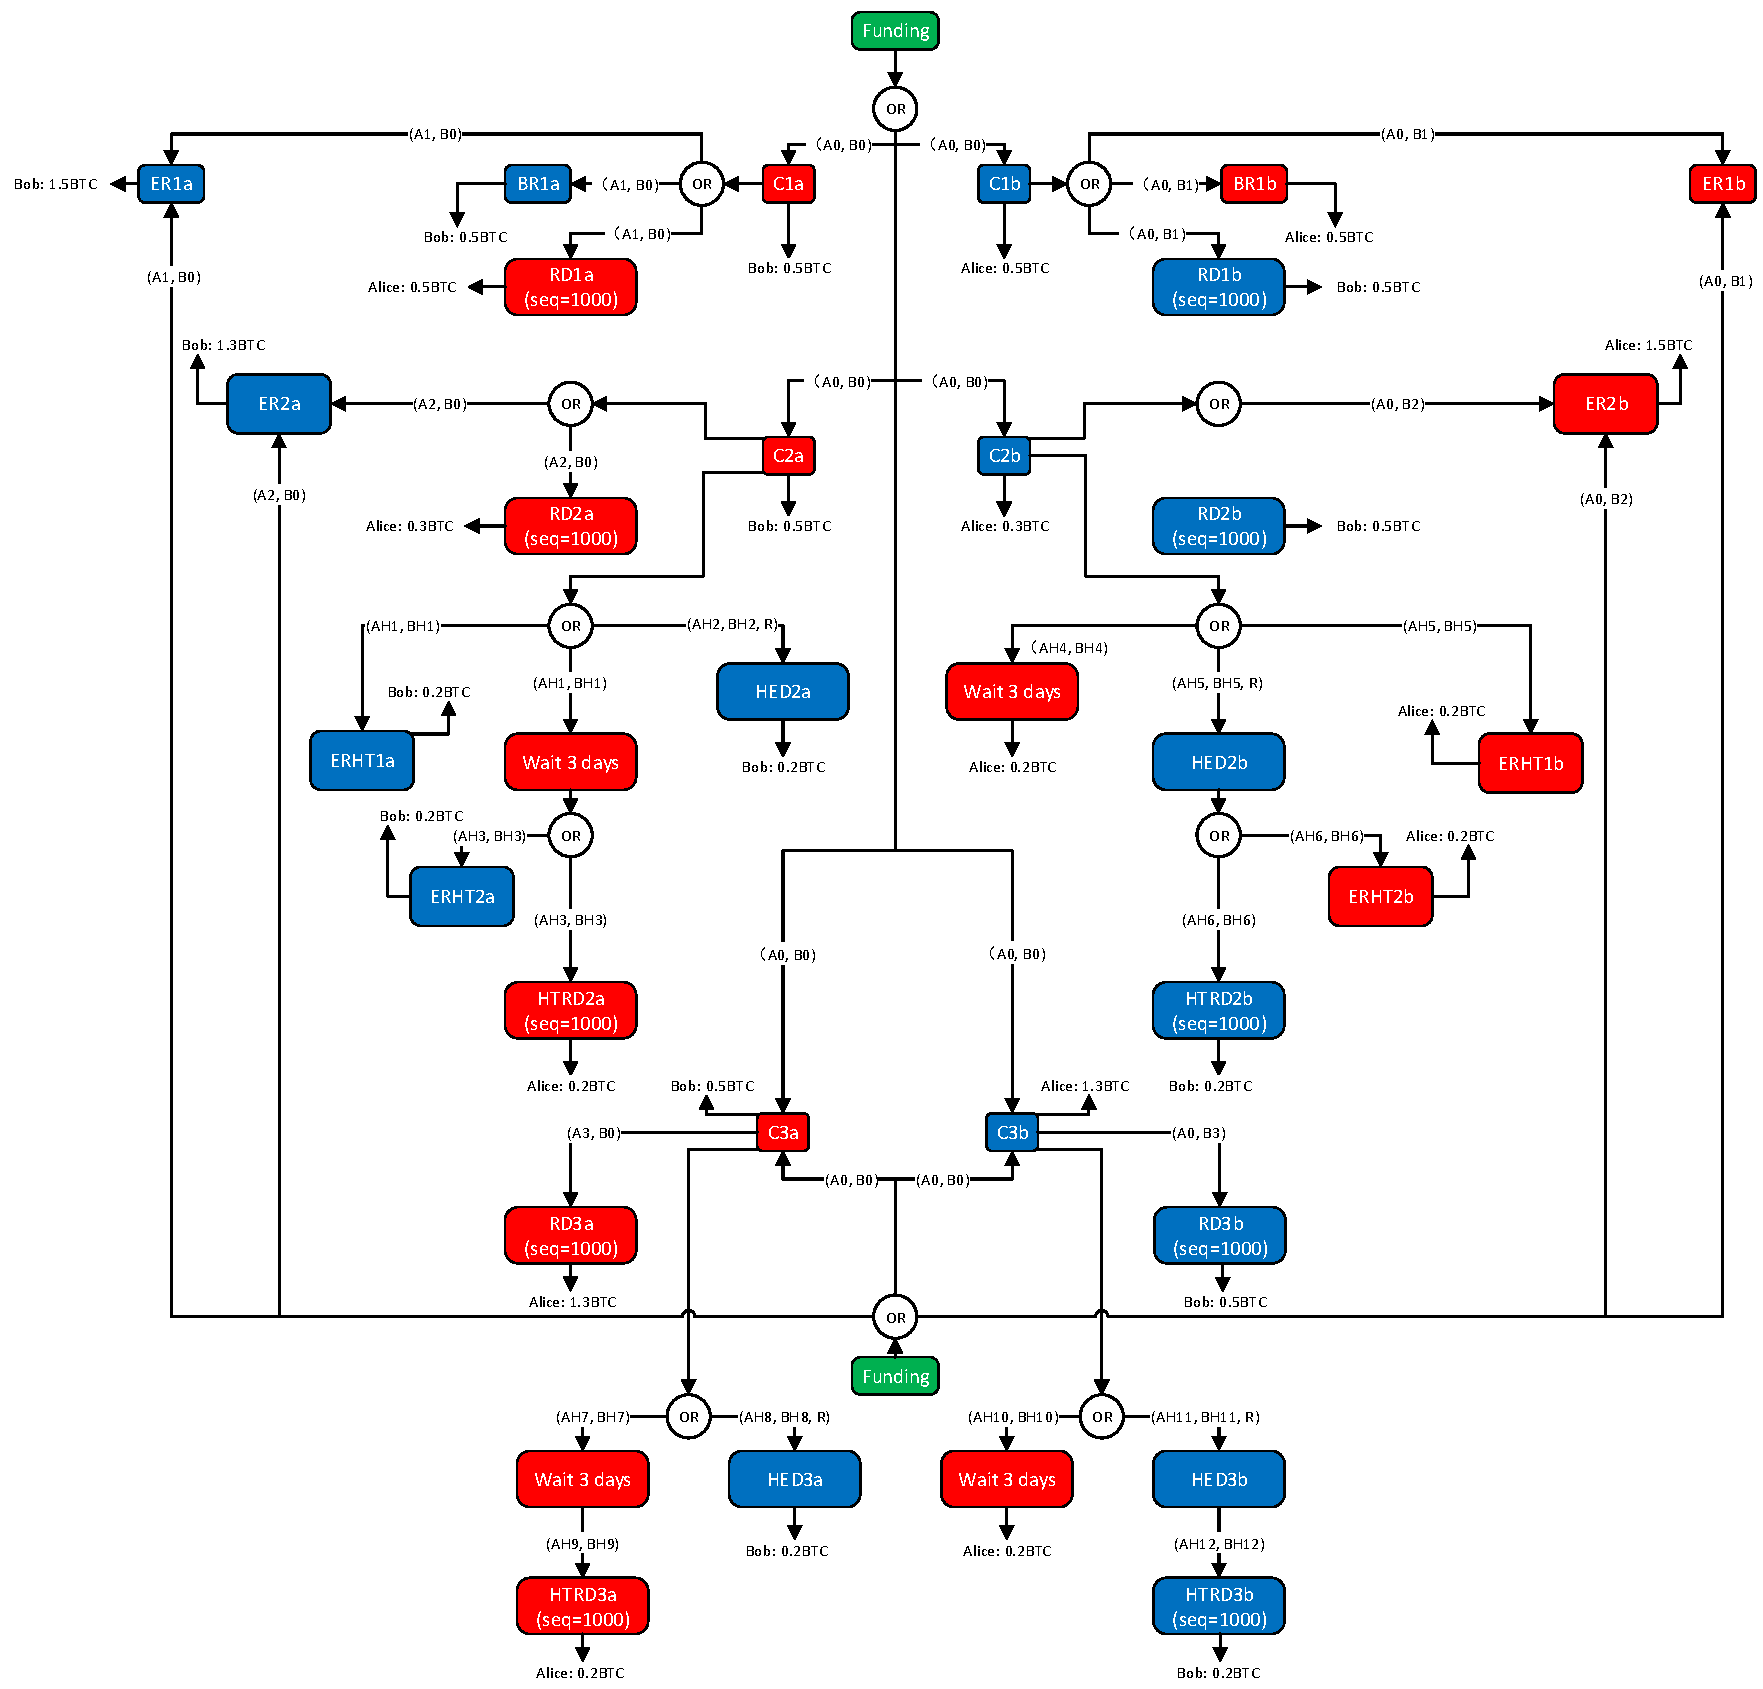
\includegraphics[width=6in]{figs/htlc_new.pdf}
\vspace{-6pt}
\caption{FundCasc HTLC transactions.}
\label{fig:htlc_new}
\end{figure}

\subsection{FundPara}


The first approach {\em FundPara} enables each new commitment to take all Funding Transactions as its input. The benefit of this approach is that all Funding Transactions are parallel: counterparties can agree on new Commitment
Transactions with arbitrary combinations of Funding Transactions as input.
Figure~\ref{fig:rsmc_new} and~\ref{fig:htlc_new} show the details of channel
deposit for RSMC and HTLC. FundPara demands the invalidation of {\em all} existing Commitment Transactions, while RSMC also invalidates old commitment transactions by exchanging private keys. Thus, numerous keys are exchanged when a channel has made a large amount of transactions, resulting in poor scalability.

\begin{figure}[t]
\centering
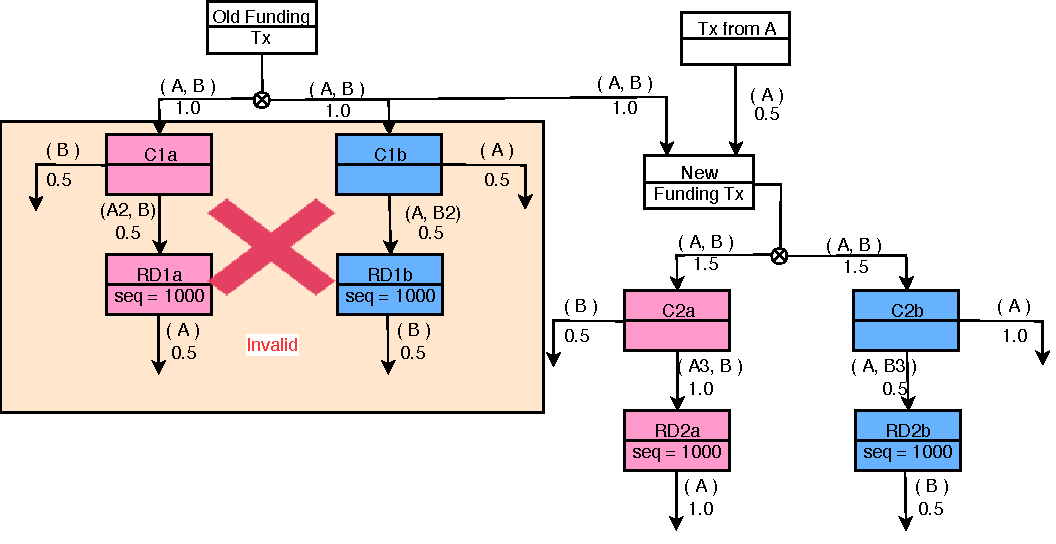
\includegraphics[width=4in]{figs/splice_in.pdf}
\vspace{-6pt}
\caption{FundCasc: Alice deposits 0.5 BTCs into the channel.}
\label{fig:splice_in}
\end{figure}

\subsection{FundCasc}


The second approach {\em FundCasc} cascades all funding transactions, i.e., the output UTXO of old Funding Transaction is directed as the "vin" of the new Funding
Transaction. Figure~\ref{fig:splice_in} depicts the solution. In Figure~\ref{fig:splice_in}, a new Funding Transaction takes two "vins:" one is the UTXO from the external transaction deposited by Alice, and the other is the UTXO from old Funding Transaction. Once the new Funding Transaction is verified on chain, all old Commitment Transactions that are derived from the old Funding Transaction become invalid. The reason is that all of them use the UTXO from old Funding Transaction as "vin", which has been spent by the new Funding Transaction. The new Funding Transaction has a "vout" with new funds in the channel. Then we use the "funding-vout" of the new Funding Transaction to create a pair of Commitment Transactions (C2a and C2b) for both participants of the channel.


Specifically, the splice-in proceeds as follows:
\begin{enumerate}
\item Creating a new Funding Transaction
\item Creating a pair of new Commitment Transactions (C2a and C2b), containing the corresponding RD2a and RD2b
\item Signing the new Commitment Transactions
\item Exchanging signatures for new Commitment Transactions
\item Signing a new Funding Transaction
\item Exchanging signatures for the new Funding Transaction
\item Broadcasting the new Funding Transaction
\end{enumerate}

\begin{figure}[t]
\centering
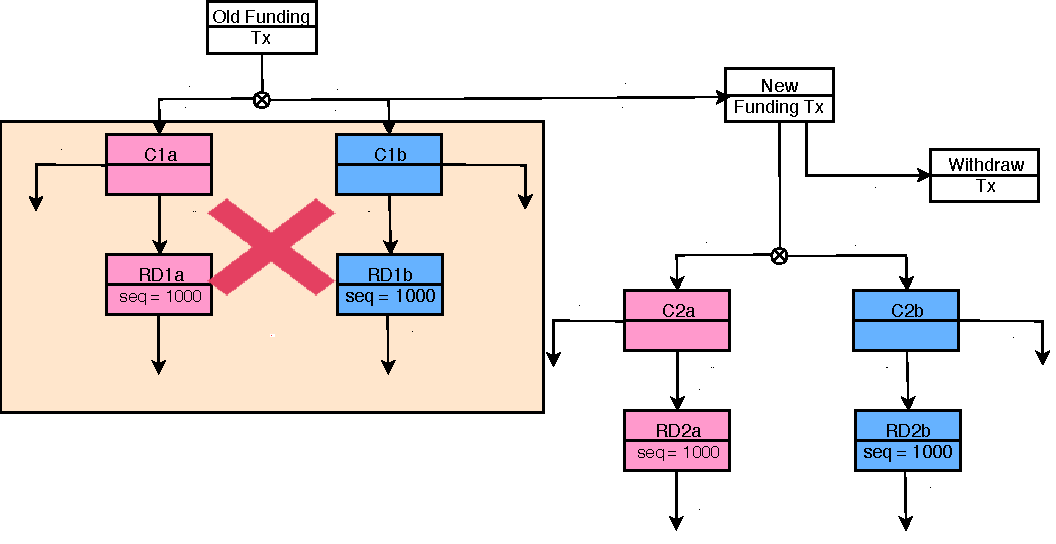
\includegraphics[width=4in]{figs/splice_out.pdf}
\vspace{-6pt}
\caption{FundCasc splice-out: Alice withdraws 0.4 BTCs from the channel.}
\label{fig:splice_out}
\end{figure}

\para{Splice-out.}
The solution of splice-out is similar to that of splice-in. Figure~\ref{fig:splice_out} shows the procedure. We construct a new Funding Transaction which takes the UTXO of an old Funding Transaction (1.0 BTC) as its only "vin". It produces two "vouts": one specifing the remaining fundings in the channel (0.6 BTCs), and the
other "vout" indicating the amount of funding withdrawn (0.4 BTCs). The remaining
fundings result in two Commitment Transactions, which corresponds to the fundings of both counterparties within the channel (0.1 BTCs for Alice and 0.5 BTCs for Bob).

\begin{figure}[t]
\centering
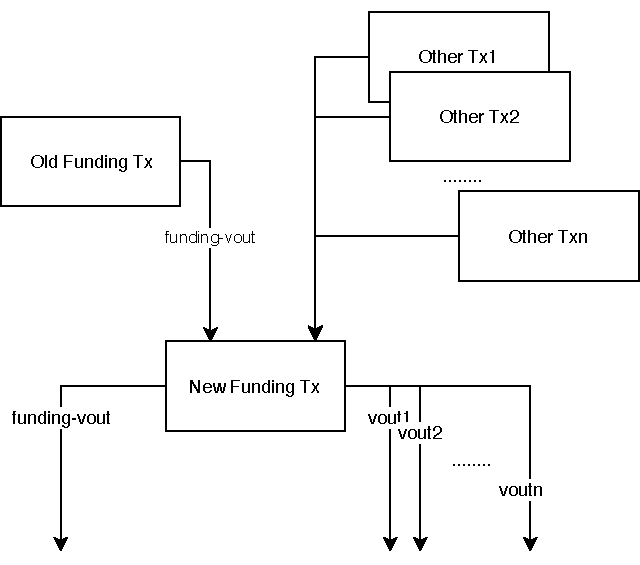
\includegraphics[width=3in]{figs/channel_change.pdf}
\vspace{-6pt}
\caption{LITEX general channel change: multiple "vins" and "vouts."}
\label{fig:change}
\end{figure}

\para{Extensions.}
The splice-in and splice-out of FundCasc have exactly one "vout" or "vin". In general, we can construct arbitrary number of "vins" and "vouts" for the new Funding Transaction whenever deemed necessary. Figure~\ref{fig:change} demonstrates a case with $n+1$ "vins" (one from previous Funding Transaction) and $n+1$ "vouts" (one from the channel).


This design brings great flexibility for channel management. For example,
Alice wants to deposit a large amount of funding into the channel but she only
has multiple small UTXO. At the same time, Bob intends to withdraw some fundings
to his various accounts. In this case, they can agree on a new Funding Transaction with multiple "vins" and "vouts".


The proposed approach is also compatible with previous approaches such as
channel rebalancing. For example, a participant can use the Circle Pay approach
to rebalance his/her fundings across multiple channel. When Circle Pay fails,
he/she may employ our proposed splice-in/splice-out approaches.


\section{Experiments}
\label{sec:eval}


\section{Conclusions}
\label{sec:conclusions}


%----------------------------------------------------------------------------
\bibliographystyle{abbrv}
\bibliography{paper}

\end{document}
